\documentclass[11pt,a4paper]{article}
\usepackage[utf8]{inputenc}
\usepackage[T1]{fontenc}
\usepackage[ngerman]{babel}
\usepackage{amsmath}
\usepackage{amsfonts}
\usepackage{amssymb}
\usepackage{graphicx}
\usepackage{packets}
\usepackage[left=2.5cm, right=2cm, top=2cm]{geometry}
\author{Lars Döpper}
\date{\today}
\title{441 Computerphysik - Hausaufgabe 3}
\begin{document}

	\maketitle
\section*{H.9: Grundzustand für (m,n)-Potentiale}
In dieser Hausaufgabe beschäftigen wir uns mit allgemeinen Potentialen der Form:
\begin{equation}
V_{m,n}(r) = V_0\left( \left(\frac{R}{r}\right)^{m} -\frac{m}{n}\left(\frac{R}{r}\right)^{n} \right)\frac{n}{m-n}
\end{equation}
Mit den Einschränkungen $V_0>0$ und $m>n$. Ziel dieser Hausaufgabe ist  die Bestimmung der Grundzustandsenergie des Lennard-Jones-Potentials mit $m=12 \; \&\; n=6$. Dazu gehen wir wieder von der zeitunabhängigen Schrödingergleichung aus:
\begin{equation}\label{eq:schrödinger}
	-\frac{\hbar^2}{2M}\Delta\phi(\vec{x}) + V(\vec{x})\phi(\vec{x}) = E\phi(\vec{x})
\end{equation}
Und setzen in diese dann das (m,n)-Potential ein und suchen nach dem ersten Eigenwert dieses Problems.
Wir interessieren uns allerdings nur für die sog. s-Wellen, also für die Wellen mit Drehimpulsquantenzahl $l=0$. Somit ist das Potential nicht mehr Richtungsabhängig und wir können das Potential im  Impulsraum schreiben als:
\begin{equation}
	V^{l=0}(p, p')=\frac{(4\pi)^2}{(2\pi)^3}\int_{0}^{\infty}r^2drV(r)\frac{\sin(pr)}{pr}\frac{\sin(p'r)}{p'r}
\end{equation}
Für allgemeine (m,n)-Potentiale müssen wir dieses Integral zumeist numerisch lösen. In dieser Hausaufgabe verwenden wir dafür die Integrationsmethode nach Gauß und Legendre.
\subsection*{9.1: Das  (2,1)-Potential}
Um unsere Methoden zu entwickeln und auf ihre Richtigkeit zu prüfen, untersuchen wir zunächst das  (2,1)-Potential.  Dieses lautet dann:
\begin{equation}\label{eq:21pot}
	V(r) = V_0\left(\left(\frac{R}{r}\right)^2 -2\left(\frac{R}{r}\right)\right)
\end{equation}
\subsubsection*{Umformung der Schrödingergleichung}
Wir wechseln jetzt in ein neues Koordinatensystem mit $\vec{y} = \vec{x}/R$. Unter Zuhilfenahme der Kettenregeln transformieren wir so unsere Schrödingergleichung. Es gilt dabei:
\begin{align*}
	\frac{\partial}{\partial x_i} &= \frac{\partial y_i}{\partial x_i}\frac{\partial}{\partial y_i} \\
	&=\frac{1}{R}\frac{\partial}{\partial y_i}
\end{align*}
Und somit weiter:
\begin{align*}
	\frac{\partial^2}{\partial x_i^2} &= \frac{\partial y_i}{\partial x_i}\frac{\partial}{\partial y_i}\left(\frac{1}{R}\frac{\partial}{\partial y_i}\right) \\
	&= \frac{1}{R^2}\frac{\partial^2}{\partial y_i^2}
\end{align*}
Für das Potential gilt zudem:
\begin{align*}
	V(x) &= V_0\left(\left(\frac{R}{x}\right)^2 -2\left(\frac{R}{x}\right)\right) \\
	&= V(x=yR) \\
	&= V_0\left(\left(\frac{1}{y}\right)^2 -2\left(\frac{1}{y}\right)\right)
\end{align*}
Mit diesen Ausdrücken können wir nun die Schrödingergleichung umformen zu:
\begin{align}
	0 &= \left[-\frac{\hbar^2}{2MR^2}\sum_{i=0}^{3}\frac{\partial^2}{\partial y_i^2}+V(y) -E\right]\Phi(yR) \\
	0 &= \left[-\frac{1}{2}\sum_{i=0}^{3}\frac{\partial^2}{\partial y_i^2} + v(y) - \epsilon\right]\Psi(y)
\end{align}
Wobei gilt:
\begin{align*}
	v_0 &= \frac{V_0MR^2}{\hbar^2} \\
	\epsilon &= \frac{E MR^2}{\hbar^2}
\end{align*}
Die Energie wird also in Einheiten von $\frac{\hbar^2}{MR^2}$ angegeben.
\subsubsection*{Potential im Impulsraum}
Wir modifizieren dieses Potential allerdings etwas, um eine Konvergenz des Integrals für beliebige p und p' sicherzustellen. Das modifizierte Potential lautet dann:
\begin{equation}
	v_{\mu}^{l=0}(y) = v_o\left[\left(\frac{1}{y}\right)^2 -\frac{2}{y}\right]e^{-\mu y}
\end{equation}
Das Potential im Impulsraum lautet dann:
\begin{equation}
	v^{l=0}(p,p') = \frac{2}{\pi}\int_{0}^{\infty}y^2dy\; v_{\mu}(y)\frac{\sin(py)\sin(p'y)}{pypy'}
\end{equation}
Dieses Integral lösen wir nun einmal numerisch und einmal analytisch und vergleichen dann die Ergebnisse. Für die numerische Integration verwenden wir die Gauß-Legendere-Methode. Für das analytische integrieren setzen wir zunächst das modifizierte Potential ein und teilen dann das Integral in zwei Unterintegrale auf. Es gibt dann nach einsetzen:
\begin{equation}
	v_{\mu}^{l=0}(p,p') = \frac{2v_0}{\pi pp'}\int_{0}^{\infty}dy \left[\frac{1}{y^2}-\frac{2}{y}\right]e^{-\mu y}\sin(py)\sin(p'y)
\end{equation}
Dieses Integral teilen wir jetzt auf und für die Unterintegrale gilt dann:
\begin{align*}
	I_1(\mu) &= \int_{0}^{\infty}dye^{-\mu y}\frac{\sin(py)\sin(p'y)}{y^2} \\
	I_2(\mu) &= -2\int_{0}^{\infty}dye^{-\mu y}\frac{\sin(py)\sin(p'y)}{y}
\end{align*}
Wir können jetzt $I_1$ und $I_2$ jeweils zwei bzw. ein mal nach $\mu$ ableiten, sodass die Nenner wegfallen. Danach können wir das Integral durchführen und wieder zwei bzw. ein mal nach $\mu$ integrieren.
Dabei gilt:
\begin{equation*}
	\int_{0}^{\infty}e^{-\mu y}\sin(py)\sin(p'y)dy = \frac{2\mu pp'}{(\mu^2+(p'-p)^2)(\mu^2+(p'+p)^2)}
\end{equation*}
Damit folgt dann für die Integrale unter Zuhilfenahme des Hinweises 2:
\begin{align}
	I_2 &= -\dfrac{\ln(\frac{(\mu^2+(p'+p)^2)}{(\mu^2+(p'-p)^2)})}{2} \\
	I_1 &= -\frac{1}{4}\left[\mu\ln(\frac{(\mu^2+(p'+p)^2)}{(\mu^2+(p'-p)^2)}) +2(p+p')\arctan\frac{\mu}{p+p'} +2(p-p')\arctan\frac{\mu}{p'-p}\right]
\end{align}
Damit ergibt sich dann für die analytische Lösung:
\begin{equation}
	v_{\mu}^{l=0}(p, p') = \frac{2v_0}{\pi pp'}\left(I_1 +I_2\right)
\end{equation}
Dies können wir noch ein wenig umformen und erhalten so die fertige analytische Lösung
\begin{equation}
\begin{split}
	v_{\mu}^{l=0}(p,p') &= \frac{v_0}{2\pi pp'}[2(p'-p)\arctan(\frac{p-p'}{\mu}) \\ &+2(p'+p)\arctan(\frac{p+p'}{\mu}) +(2+\mu)\left(\ln(1+\frac{(p-p')^2}{\mu^2}) -\ln(1+\frac{(p+p')^2}{\mu^2})\right) ]
\end{split}
\end{equation}
Wir vergleichen jetzt die analytische Lösung mit der numerischen Lösung und lassen uns den maximalen relativen Fehler in Abhängigkeit der Anzahl der Stützstellen $n_y$ ausgeben. Es ergeben sich die folgenden Werte:
\begin{table}[htbp]\begin{center}
		\begin{tabular}{c|c}
		$n_y$ & maximaler relativer Fehler \\ \hline
		100	&   3.553726e-01 \\
		1000	 &  2.788099e-04 \\
		10000	 &  2.788130e-04 \\
		100000	&   2.788146e-04 \\
	\end{tabular}
	\caption{Relativer Fehler der numerischen Integration}
	\end{center}

\end{table}
Wir sehen, dass der Fehler für $n_y \geq 1000$ nicht mehr signifikant sinkt, deswegen wählen wir ab jetzt $n_y=1000$ als unsere Diskretisierung für die Berechnung des Potentials im Impulsraum. Die gleiche Relation kann man auch in Abbildung \ref{fig:rel_error} sehen.
	\begin{figure}[htbp]
	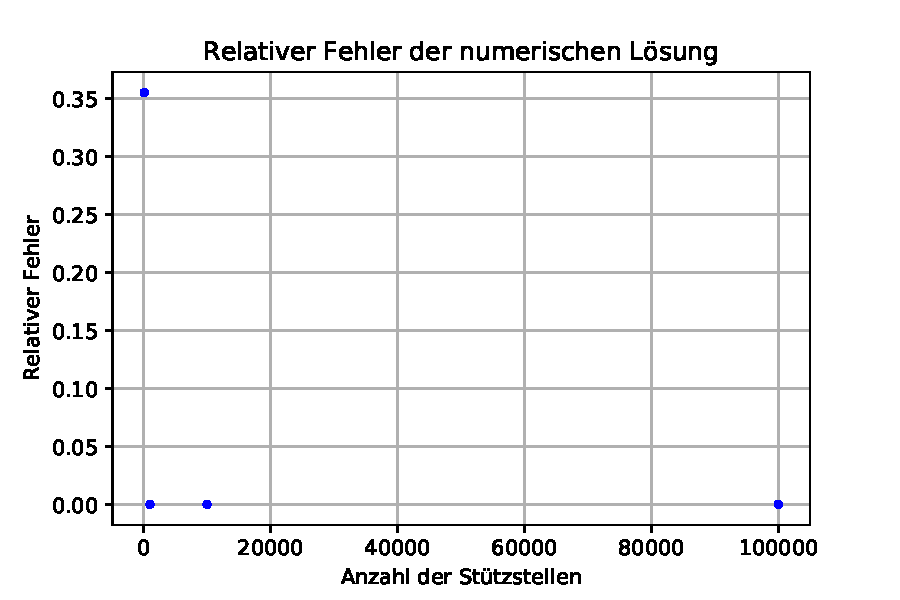
\includegraphics[width=0.9\textwidth]{9_3_relative_abweichung.pdf}\label{fig:rel_error}
	\caption{Relativer Fehler der numerischen Integration.}
	\end{figure}
\subsubsection*{Berechnung der Grundzustandsenergie}
Jetzt verwenden wir das Arnoldi-Verfahren, um die Grundzustandsenergie dieses Potentials zu bestimmen.
Für die Parameter $\mu=1$, $v_0=400$, $n_y = 1000$, $n_p = 400$ und $p_{max} = 200$ ergeben sich die numerischen und analytischen Lösungen jeweils zu:
\begin{equation}
	\epsilon_{numerisch} = -149,532
\end{equation}
\begin{equation}
	\epsilon_{analytisch} = -149,533
\end{equation}
Wir sehen also, dass diese Werte sehr nahe beieinander sind. Jetzt variieren wir die Anzahl der Stützstellen $n_y$ und $n_p$ und den Maximalimpuls $p_{max}$. Für jede Varaioton berechnen wir jeweils den maximalen relativen Fehler und geben diesen graphisch aus. Die Graphen der Fehler sieht man in Abbildung \ref{fig:rel_errors}.
\begin{figure}[htbp]
	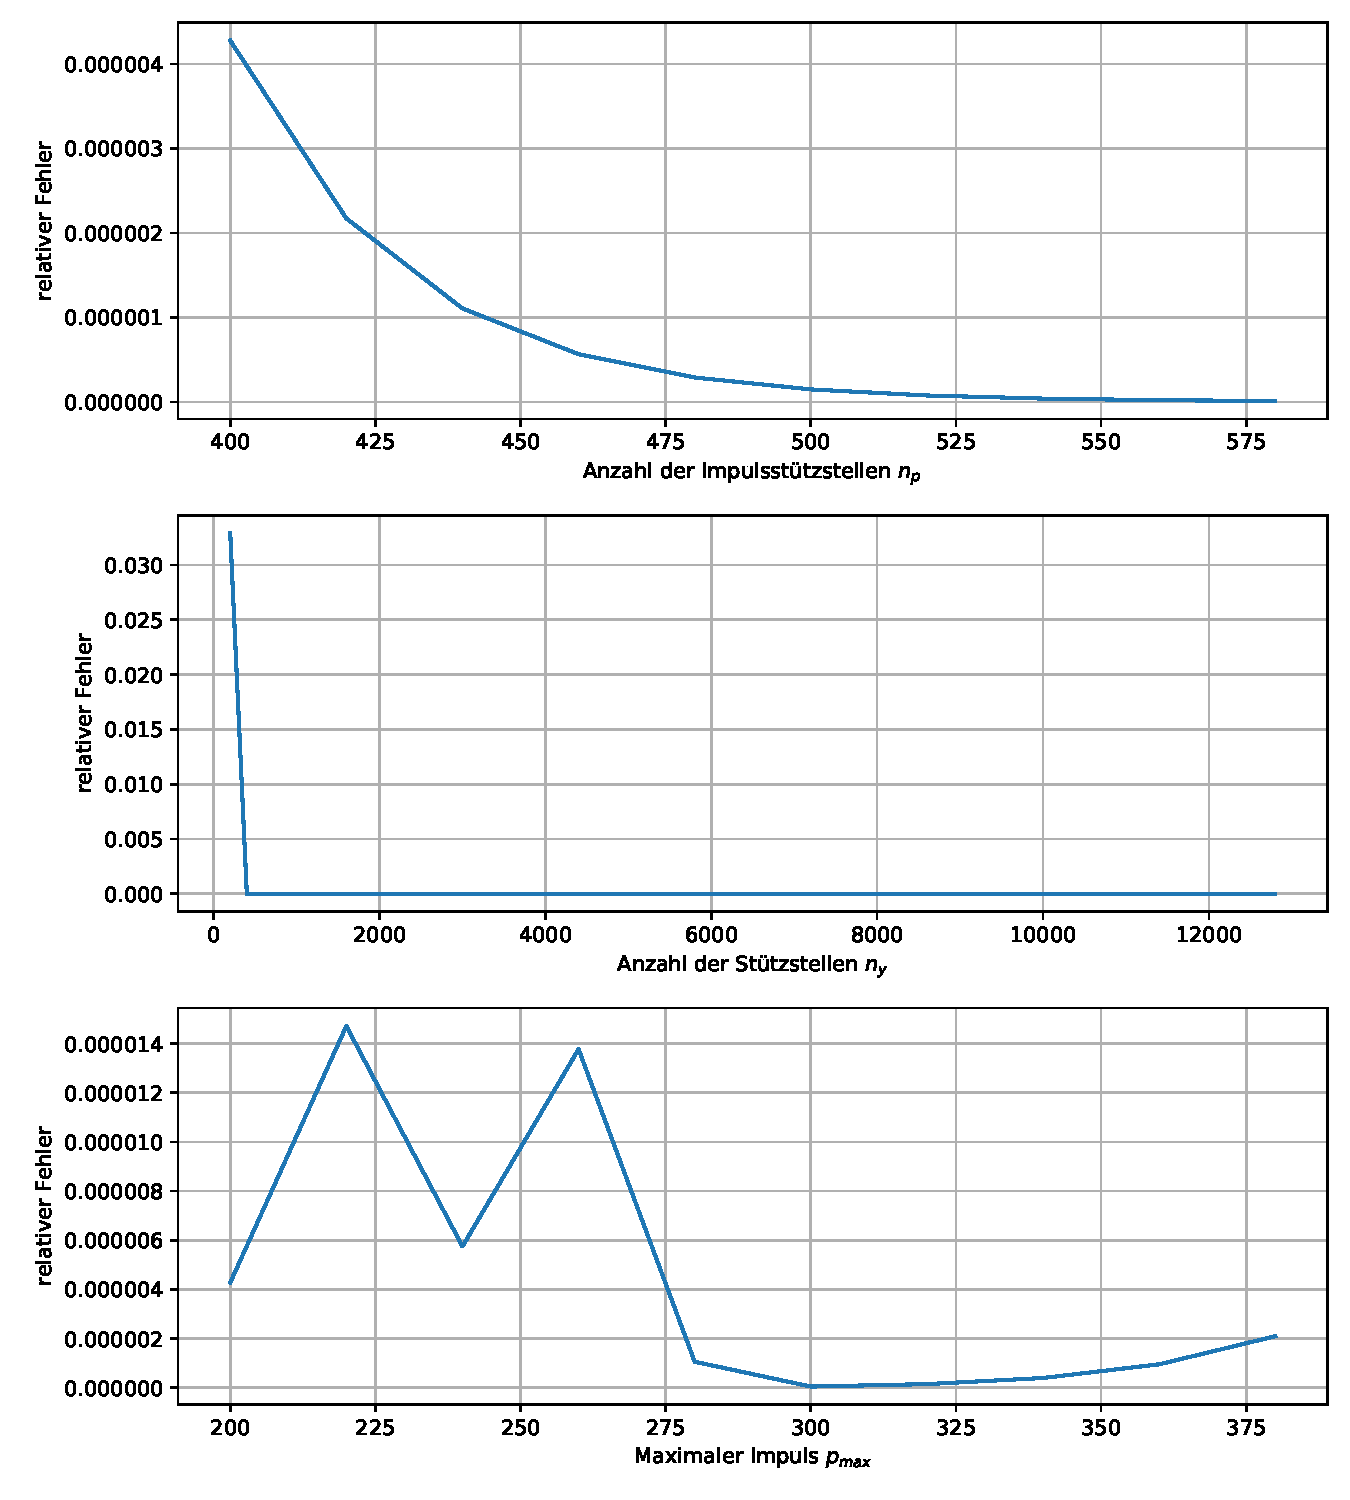
\includegraphics[width=0.9\textwidth]{rel_error_params.pdf}\label{fig:rel_errors}
	\caption{Verlauf der Relativen Fehler bei Variation der Parameter.}
\end{figure}
Man kann aus den Graphen erkennen, dass die relativen Fehler für die Anzahl der Stützstellen $n_y$ sehr schnell klein werden und sich dann nicht mehr stark unterscheiden. Für die Anzahl der Impulsstellen $n_p$ fällt der relative Fehler exponentiell ab. Zuletzt lässt sich für $p_{max}$ kein klares Muster erkenne, allerdings sinkt der relative Fehler ab $p_{max} = 270$ stark und bleibt danach auch sehr klein.

Hier noch Tabellen einfügen für Fehler.
\subsubsection*{Harmonische Näherung}
Wir entwickeln nun das Potential im Ortsraum in einer Taylorreihe und bestimmen aus der Näherung bis zur Ordnung $y^2$ die Grundzustandsenergie verglichen mit dem harmonischen Oszillator.
\subsection*{9.2: Das Lennard-Jones-Potential}
In diesem Aufgabenteil wenden wir unsere Erkenntnisse aus dem (2,1)-Potential auf das Lennard-Jones-Potential mit (12,6) an.
\subsubsection*{Das numerische Potential}
 Zunächst berechnen wir numerisch den Wert des Potentials im Impulsraum. Wir haben als Parameter $p'=1$,$p_{max}=400$, $y_{min}=0.4$ und $n_y = 20000$ gewählt.Den Verlauf sieht man in Abbildung \ref{fig:lennard_jones_pot}.
\begin{figure}[htbp]
	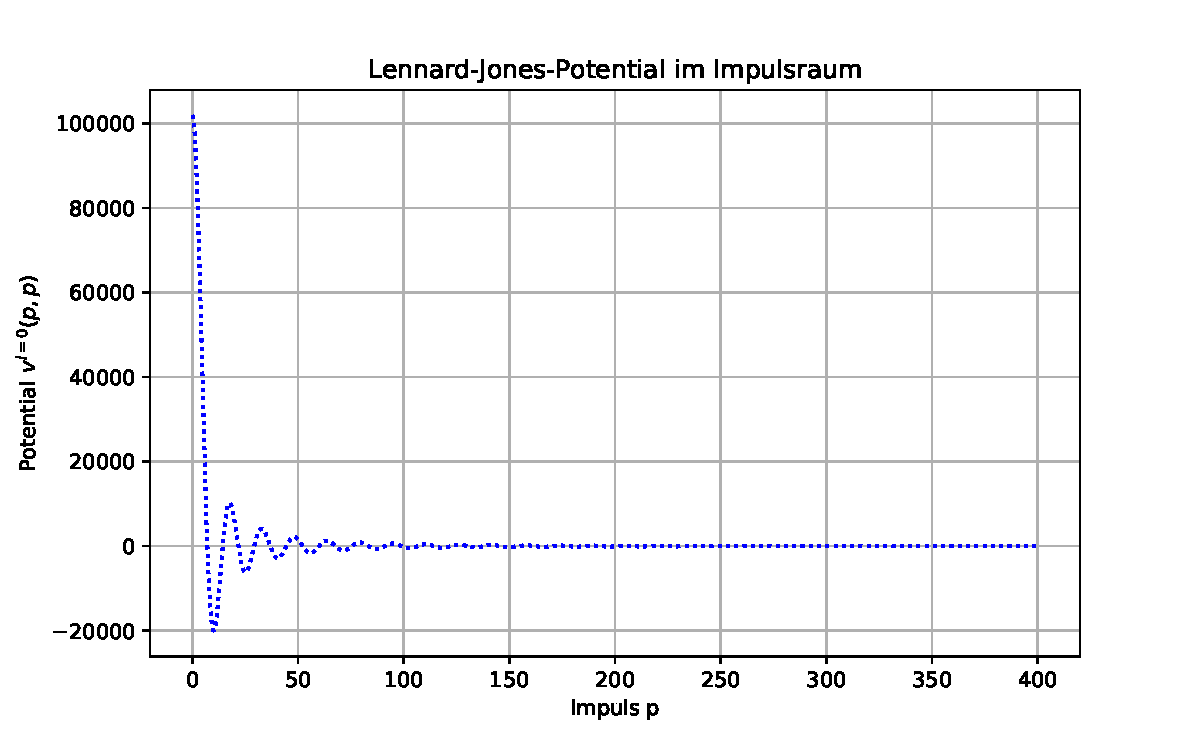
\includegraphics[width=0.9\textwidth]{lennard_jones_pot.pdf}\label{fig:lennard_jones_pot}
	\caption{Verlauf des Lennard-Jones-Potentials im Impulsraum}
\end{figure}
\subsubsection*{Die Grundzustandsenergie}
Wir verwenden wieder das Arnoldi-Verfahren, um die Grundzustandsenergie zu finden.
\subsubsection*{Harmonische Näherung}
Wir entwickeln das Lennard-Jones-Potential in einer Taylorreihe bis zur Ordnung $y^2$ und vergleichen dieses mit dem Potential des harmonischen Oszillator.
\newpage
\listoffigures
\end{document}